\appendix
%\appendixpage
\addappheadtotoc
\chapter{所用诊断模型细节}
\label{ch:appendix}

本文使用了现有云中医技术作为技术探针,在其基础上进行了开发。
云中医由复旦大学计算机学院和上海中医药大学合作研制,
其模型处理流程如图\ref{fig:cloudmed2}所示,面部图片、舌部图片和用户对健康问题的回答作为模型输入,经过人脸检测、区域提取算法将图片进行预处理,截取肤色、唇部、舌部区域,通过由人工标记数据训练过的SVM分类器得到更加细粒度的特征。
最后,由专家编写的诊断规则将上述过程得到的特征和用户对健康问题的回答,转化为用户的健康得分和体质倾向。

\begin{figure}[htb]
    \centering
    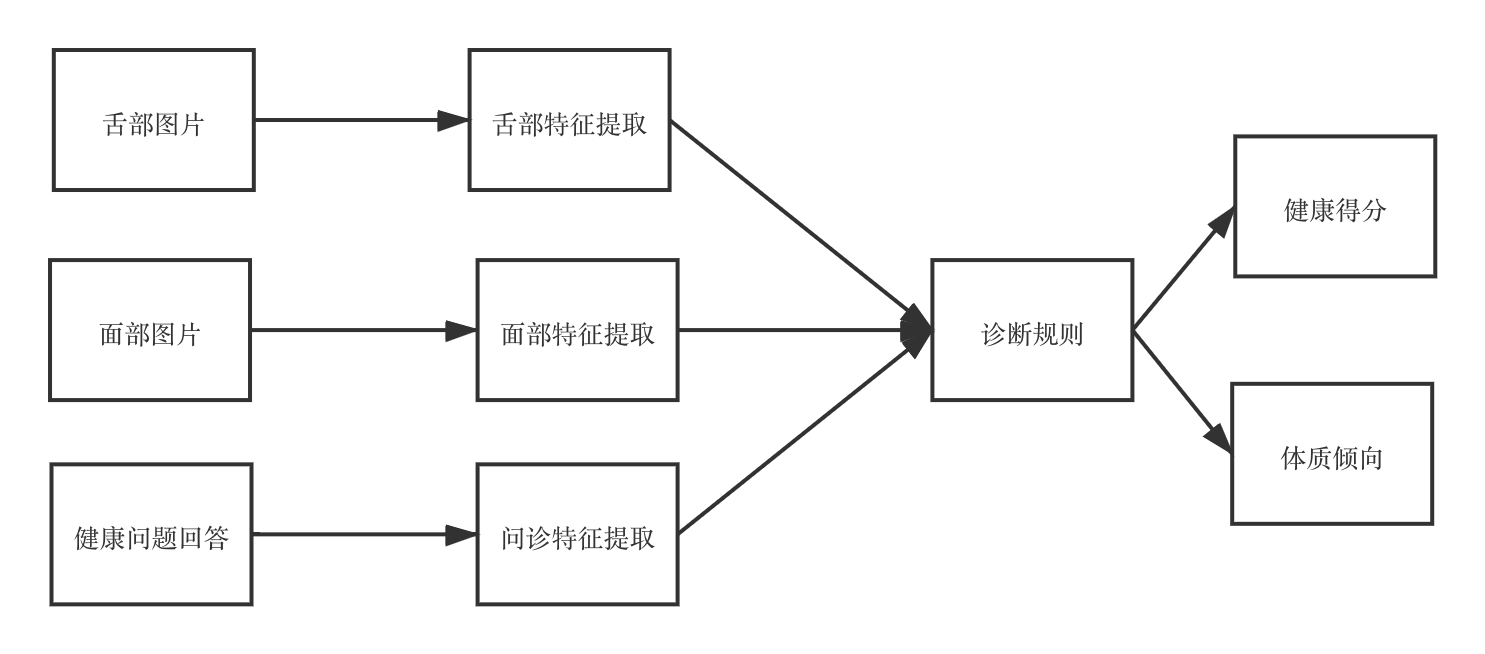
\includegraphics[width=15cm]{images/cloud_med3.png}
    \caption{技术探针模型处理流程}
    \label{fig:cloudmed2}
\end{figure}

下文将分别从面部特征提取、舌部特征提取、问诊特征提取、诊断规则四个部分介绍处理过程与使用的算法。

\section{面部特征提取}
\label{subsec:face_feature}

\begin{table}[h]
    \centering
    \caption{面部特征提取}
    \begin{tabular}{lll}
        \toprule
        特征          & 特征描述     & 特征内容 \\
        \midrule
        faceDetectRes & 检测到人脸   & 0:未检测出人脸、1:成功检测出人脸  \\
        faceColor     & 面部颜色 & 0:面白,1:面黑、2:面红、3:面黄、4:面青、5:正常 \\
        faceGloss     & 面部光泽 & 0:有光泽、1:少光泽、2:无光泽\\
        lipDetectRes  & 检测到嘴唇   & 0:未检测出嘴唇、1:成功检测出嘴唇\\
        lipColor      & 嘴唇颜色 & 0:淡白、1:淡红、2:红、3:暗红、4:紫   \\
        \bottomrule
    \end{tabular}
    \label{tab:face-feature}
\end{table}

如表\ref{tab:face-feature}所示,在面部特征提取阶段,输入为面部图片,输出有以下几个维度:
 \begin{enumerate}
     \item 检测到人脸(faceDetectRes):如果没有检测到人脸,则剩余所有维度无效,且取值为0。

     \item 检测到嘴唇(lipDetectRes):如果没有检测到嘴唇,嘴唇颜色的结果无效且取值必定为0。

     \item 面部颜色、面部光泽(faceColor、faceGloss):面色和光泽是对预处理之后的图片,去除眼口鼻区域的图片进行面色和光泽信息提取的结果。

     \item 嘴唇颜色(lipColor):嘴唇颜色的结果从浅到深分别为淡白、淡红、红、暗红、紫。
\end{enumerate}

\begin{figure}[htb]
    \centering
    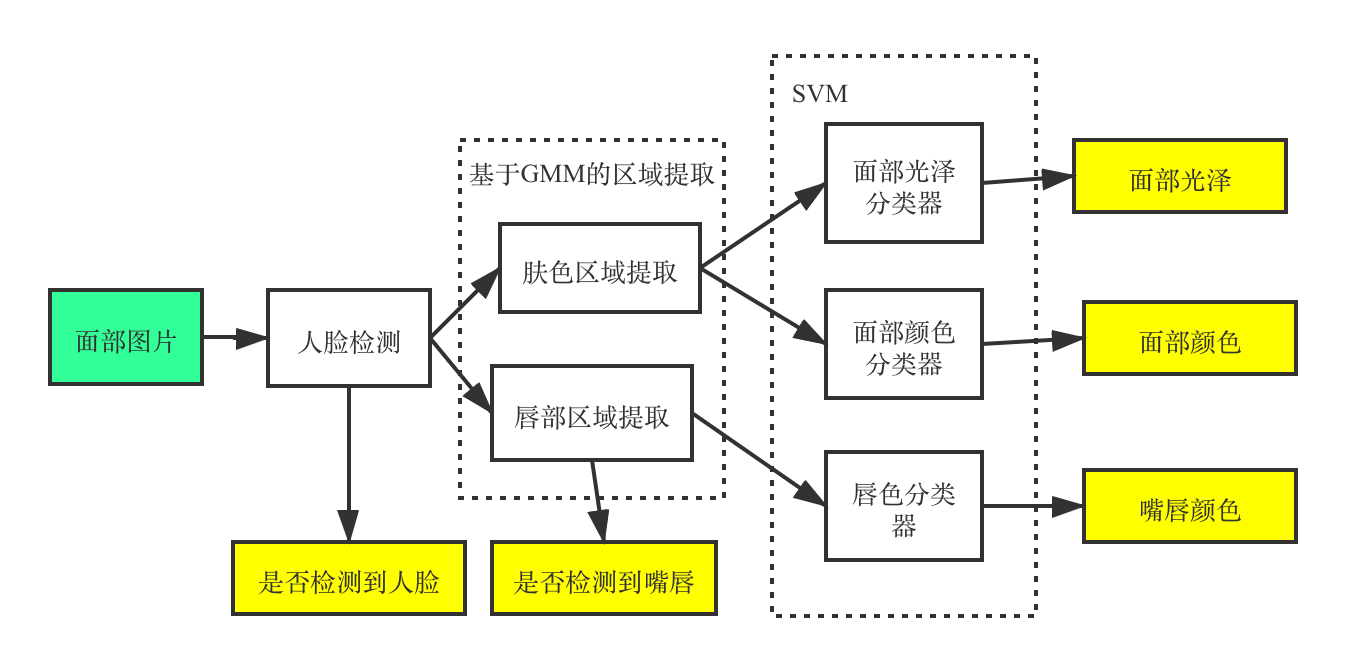
\includegraphics[width=15cm]{images/face_feature.png}
    \caption{面部特征提取}
    \label{fig:face_feature}
\end{figure}

表\ref{tab:face-feature}中对应的特征,产出流程如图\ref{fig:face_feature}所示,其中绿色代表输入,黄色代表产出特征:
(1)首先使用人脸检测算法,判断是否存在人脸,并截取人脸区域;
(2)利用基于混合高斯模型(GMM)的区域提取方法\cite{Hu2016Robust},截取人脸区域中的面部区域与唇部区域;
(3)经过若干特征工程得到颜色特征,通过多个SVM分类器将这些特征分类为具体的面部特征,如面部光泽、面部颜色、嘴唇颜色等。


\subsection{基于混合高斯模型的区域提取方法}

高斯分布也称为正太分布,是自然界大量存在的最为常见的分布模式。

\begin{equation}
\label{eq:equation1}
    \mathcal{N}(x | \mu, \Sigma) = \frac{1}{(2\pi)^{D/2}}\frac{1}{|\Sigma|^{1/2}}exp\{-\frac{1}{2}(x-\mu)^T\Sigma^{-1}(x-\mu)\}
\end{equation}

混合高斯模型是对高斯分布模型的拓展,假设数据的分布为多个高斯分布的线性叠加组成,相比简单高斯分布对复杂数据的刻画能力更强。
\begin{equation}
\label{eq:equation2}
p(x) = \Sigma^K_{k=1}\pi_k\mathcal{N}(x|\mu_k,\Sigma_k)
\end{equation}
其中
\begin{equation}
\label{eq:equation3}
\Sigma^K_{k=1}\pi_k = 1
\end{equation}

混合高斯模型在图像处理中经常用来完成图像分割任务:通过对图像中的像素点进行混合高斯模型建模,可以得到图像上每个点属于某个高斯模型的概率,进而通过概率值将图像分割为多个区域。


利用混合高斯模型进行兴趣区域提取,可以截取唇部区域,如研究\cite{Hu2016Robust}所述主要步骤如下:
\begin{enumerate}
    \item 使用人脸检测算法检测图片中是否包含人脸,裁剪人脸区域作为下一步输入。

    \item 对人脸上半部分无唇部的区域使用混合高斯模型获取当前图像的肤色概率分布p。

    \item 根据经验值,预先设置好肤色裁剪比例参数列表\textit{it[N]}。

    \item 迭代式地判断\textit{N}次,对于每次迭代\textit{i},在人脸下半部分定位唇部:(1)按照预先设置的参数\textit{it[i]},通过比较每个像素点的肤色概率\textit{p[x]}和参数\textit{t[i]}, 如果\textit{p[x]>t[i]}, 去除皮肤区域。最终得到去除部分肤色区域的图像。
(2)在图像中根据唇部的形状与色彩特征,定位到唇部个数:如果个数为1标记为找到唇部区域,继续迭代;否则标记为未找到唇部区域,直接退出。

    \item 在上一步获取到的有唇部区域的图像中,按照图像中的肤色区域大小变化率绘制曲线,取曲线的局部最小值对应的唇部区域作为最终的唇部裁剪区域。

    \item 对唇部轮廓进行简化平滑处理,截取出唇部区域。
\end{enumerate}

在上述方法中,\textit{N}为迭代次数,一般设置为14,裁剪比例参数为\{0.6, 0.5, 0.4, 0.3, 0.2, 0.1, 0.05, 0.01, 0.005, 0.001, 0.0005, 0.0001, 0.00005, 0.00001\}。
如研究\cite{Hu2016Robust}中所述,通过对1131张从曙光医院拍摄的人脸数据集进行验证,该方法在检测唇部区域时的区域覆盖率能达到96.76\%,对有胡子的人脸也能很好地分割唇部。

\subsection{基于SVM的特征提取方法}
基于颜色模型,技术探针采取研究\cite{Hu2016Robust, Zhao2014Qualitative}中的方法提取唇色、面色特征。
以提取面色特征为例,首先将混合高斯模型提取的肤色区域图片映射到LAB颜色空间得到LAB特征,如算法\ref{alg:face-color-feature}所示,在经过去噪处理后,取颜色的平均值作为面部颜色特征:
(1)如果L>165,面色特征为面白;(2)如果L<125,面色特征为面黑;(3)将A、B特征使用SVM分类器进行训练,得到面色特征分类。
如研究\cite{Zhao2014Qualitative}中述,通过对曙光医院采集的877张人脸图片进行面色分类与5位专业医生给出的结果进行对比验证,对于面红和正常准确率达到90\%以上,面白判断准确率为74\%,其他面色判断准确率为80\%左右。

\begin{algorithm}[htbp]
    \caption{extractFaceSkinColorFeature 面色特征提取\cite{Zhao2014Qualitative}}%算法名字
    \label{alg:face-color-feature}
    \LinesNumbered %要求显示行号
    \KwIn{faceImage 肤色区域图片}%输入参数
    \KwOut{faceSkinColorFeature 面部颜色空间像素特征}%输出
    faceImageGray = 灰度图像(faceImage)\\

    \tcc{进一步去除一些明暗的像素}
    \For{像素点 in faceImageGray} {
        \If{像素点亮度大于图中2\%的点} {
            从faceImage中去除该点
        }
        \If{像素点亮度小于图中10\%的点} {
            从faceImage中去除该点
        }
    }
    faceSkinColorFeature = 像素点平均值(faceImage)\\
    \Return{faceSkinColorFeature}\\
\end{algorithm}

在提取面部光泽部分,通过截取面部图片的子区域(裁剪矩形比例为{0.65, 0.5, 0.6, 0.35}),得到右边脸颊的图像区域,以右边脸颊的HSV颜色空间特征,训练SVM分类器得到面部光泽特征。
该方法通过对从医院获取并经过专家判别的60张有光泽面部图片与60张无光泽面部图片进行实验,在HSV颜色空间下最高达到84\%的准确率。
%
%部分代码如下所示:
%
%\begin{lstlisting}[language={C}, title=面色特征提取代码, label={lst:extract-face-color}]
%CvScalar FaceSkinDetectionByGMM::extractFaceSkinColorFeature()
%{
%	//获得灰度图像
%	IplImage* faceImageGray = cvCreateImage(cvGetSize(faceImage),8,1);
%	cvCvtColor(faceImage,faceImageGray, CV_BGR2GRAY);
%
%	//进一步去除一些明暗的像素
%	int i_dark,i_bright;
%	double rate_dark = 0.1, rate_bright = 0.02;
%	calculateDarkAndBrightThreshold(faceSkinMask,faceImageGray,i_dark,i_bright,rate_dark,rate_bright);
%	for (int y=0;y<faceSkinMask->height;++y)
%	{
%		for (int x=0;x<faceSkinMask->width;++x)
%		{
%			if (cvGetReal2D(faceImageGray,y,x)<i_dark || cvGetReal2D(faceImageGray,y,x)>i_bright)
%			{
%				cvSetReal2D(faceSkinMask,y,x,0);
%			}
%		}
%	}
%
%	CvScalar faceSkinColorFeature = cvAvg(faceImage_Lab,faceSkinMask);
%	return faceSkinColorFeature;
%}
%\end{lstlisting}
%
%\begin{lstlisting}[language=C, title=唇部光泽特征提取代码, label={lst:extract-lip}]
%CvScalar LipSegmentation::ExtractLipColorFeature(){
%    //获得灰度图像
%    IplImage* lipImageGray =
%        cvCreateImage(cvGetSize(lipImage),8,1);
%    cvCvtColor(lipImage,lipImageGray, CV_BGR2GRAY);
%
%    //进一步去除一些明暗的像素
%    int i_dark,i_bright;
%    double rate_dark = 0.2, rate_bright = 0.02;
%    calculateDarkAndBrightThreshold(lipRawMask,lipImageGray,i_dark,
%        i_bright,rate_dark,rate_bright,0);
%    for (int y=0;y<lipRawMask->height;++y){
%        for (int x=0;x<lipRawMask->width;++x){
%           if(cvGetReal2D(lipImageGray,y,x)<i_dark || cvGetReal2D(lipImageGray,y,x)>i_bright){
%                cvSetReal2D(lipRawMask,y,x,0);
%            }
%        }
%    }
%    cvErode(lipRawMask,lipRawMask);
%    RemoveNoise rn;
%    rn.LessConnectedRegionRemove(lipRawMask, lipRawMask->height*lipRawMask->width/30);
%
%    // 转换到LAB颜色空间
%    IplImage* lipImage_Lab = cvCreateImage(cvGetSize(lipImage),8,3);
%    cvCvtColor(lipImage,lipImage_Lab, CV_BGR2Lab);
%
%    // 取像素平均值作为特征
%    CvScalar lipColorFeature = cvAvg(lipImage_Lab,lipRawMask);
%
%    return lipColorFeature;
%}
%\end{lstlisting}
%
%\begin{lstlisting}[language={C}, title=面色特征SVM分类代码, label={lst:predict-face-color}]
%int FaceComplexionRecognition::colorPredict(const CvScalar skinColor) {
%    int response = 5;
%    float L;
%    // 提取特征
%    float feature[2];//<a,b>
%    L = skinColor.val[0];
%    feature[0] = skinColor.val[1];//a
%    feature[1] = skinColor.val[2];//b
%
%    if (L>=165) {
%        response = 0;//白
%    } else if (L<=125) {
%        response = 1;//黑
%    } else {
%        Mat featureMat(1,2,CV_32FC1,feature);  //特征数据
%        //预测
%        CvSVM svm = CvSVM();
%        svm.load(colorClassifierPathName);
%        response = (int)svm.predict(featureMat);
%    }
%    return response;
%}
%\end{lstlisting}
%
%由于涉及的特征比较多,大部分特征提取的代码基本结构类似,在后续内容中特征的提取与分类过程主要以伪代码和文字描述为主进行阐述。


\subsection{面部诊断规则}

\begin{algorithm}[htbp]
    \caption{getFaceScore 获取面部诊断结果\cite{张红凯2018基于舌}}%算法名字
    \label{alg:face_score}
    \LinesNumbered %要求显示行号
    \KwIn{面部特征faceResult}%输入参数
    \KwOut{score数组,对应7种体质倾向分数}%输出
    score = new Array(7) \\

    \If{faceResult.faceDetectRes==检测到人脸}{
        \If{faceResult.面色 == 白色}{
            \tcc{阳虚分数增加}
            score[0] += 5\\
            \tcc{肾虚分数增加}
            score[5] += 8\\
        }
        \If{faceResult.面色 == 黄色}{
            \tcc{脾虚分数增加}
            score[4] += 10\\
        }
        \ldots\\
    }
    \Return{score}\\
\end{algorithm}

面部诊断规则主要是为后续诊断规则部分提供体质倾向得分。
如算法\ref{alg:face_score}所示,诊断规则将面部特征结果经过预定义的规则,将其映射到一个大小为7的score数组中。
score数组代表对于阳虚、阴虚、痰湿、瘀滞、脾虚、肾虚、气虚7类体质的倾向,初始化为全0。
如果面部特征提取的面色为白色,则会导致阳虚分数增加5分、肾虚分数增加8分;如果面色偏黄色,则脾虚分数将增加10分等。
在经过所有规则判断后,将score数组返回由诊断规则统一处理。
在面诊规则中,某类体质分数的增加,并不一定会代表偏向某一类体质,后续会有整体的规则对分数进行权重调整和判断。


\section{舌部特征提取}
\label{subsec:tongue-feature}

\begin{table}[h]
    \centering
    \caption{舌部特征提取}
    \begin{tabular}{lll}
        \toprule
        特征 & 特征描述 & 特征内容 \\
        \midrule
        tongueDetectRes & 检测到舌体 & 0:未检测出舌像、1:成功检测出舌像 \\
        tongueCrack & 舌裂纹 & 0:未检测到裂纹、1:成功检测到裂纹 \\
        tongueFatThin & 舌胖瘦 & 0:正常(瘦)、1:胖舌 \\
        tongueCoatThickness & 舌苔厚薄 & 0:薄、1:厚 \\
        tongueCoatColor & 舌苔颜色 & 0:苔白、1:苔黄 \\
        \multirow{2}{*}{tongueNatureColor} & 舌质颜色 & 0:舌暗红、1:舌淡白、     \\ \cline{3-2}
                                            &        & 2:舌淡红、3:舌红、4:舌紫    \\ \hline
        \bottomrule
    \end{tabular}
    \label{tab:tongue-feature}
\end{table}

如表\ref{tab:tongue-feature}所示,舌部特征提取模型,输入为舌头图片,输入有以下几个维度:
\begin{enumerate}
    \item 是否检测到舌体(tongueDetectRes):如果没有检测到舌体,则剩余所有维度无效,且取值为0。

    \item 是否检测到舌裂纹(tongueCrack):舌裂纹是最终特征,剩余特征是否有效和该标志位没有关系。

    \item 舌头特征(tongueFatThin、tongueCoatThickness、tongueCoatColor、tongueNatureColor):包括舌胖瘦,舌苔的厚薄、颜色和舌质颜色。

\end{enumerate}

\begin{figure}[htb]
    \centering
    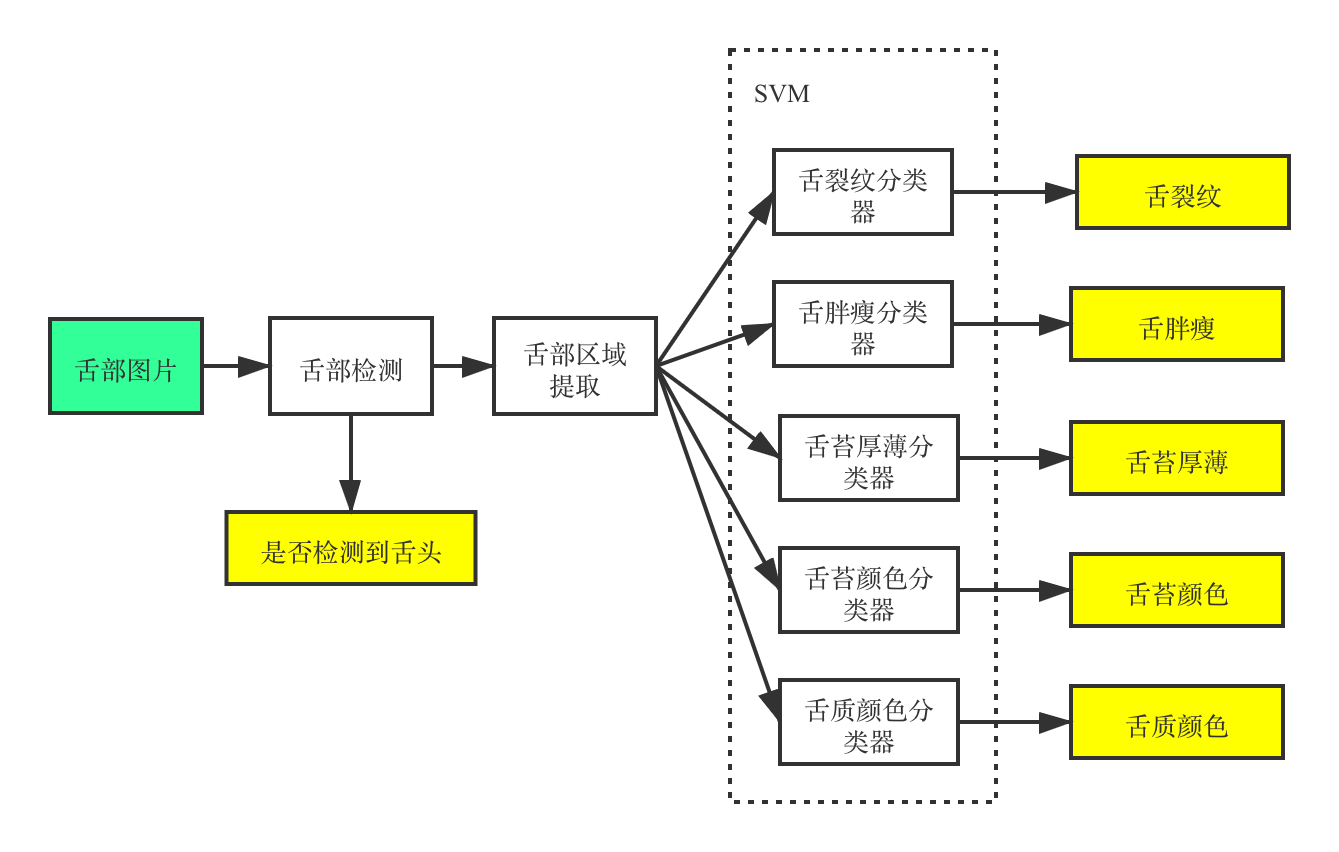
\includegraphics[width=15cm]{images/tongue-feature.png}
    \caption{舌部特征提取}
    \label{fig:tongue_feature}
\end{figure}

如图\ref{fig:tongue_feature}所示,舌部特征提取方法与面部特征提取所用方法基本相同(即通过混合高斯模型进行区域分割,然后做特征工程利用SVM分类器提取特征),此处不再赘述。
但其中检测舌体与舌裂纹方面,技术探针使用了研究\cite{zhang2018computer}中的方法,在此做简单介绍。

\subsection{舌体检测}
舌体属于图像中的连续区域,与肤色有类似的颜色分布,但具有特定的轮廓特征,技术探针使用了基于Haar特征级联分类器的方法\cite{zhang2018computer}判断图像中是否存在舌头以及分割舌部区域。
该分类器使用了900张带有舌部的照片作为正样本(标记目标位置),600张人脸照片和2000多张风景照片作为负样本训练而来,对是否存在舌部的判断准确率达到89\%\cite{zhang2018computer};
在截取舌部矩形区域后,通过混合高斯模型切割舌部区域;最后,通过截取区域内部最大矩形区域作为舌体区域用于后续特征提取。

\subsection{舌裂纹提取}
在舌裂纹提取方面,采用导向滤波器(Guided Filter)\cite{he2010guided}对原始图像对应的灰度图像进行滤波。
导向滤波器能在平滑图像的同时保留图像中的边缘特征,从而将图像中边缘部分划分为灰度值更高的部分,其他部位为灰度值较低部分。

由于舌裂纹之间宽度不一,如研究\cite{zhang2018computer}所述,采用基于模拟水流的方法,在边缘部分释放若干水分子,水分子将随机从灰度值较低部分流向灰度值较高了位置,
从而水分子将聚集在舌裂纹部位得到舌裂纹信息。

\subsection{舌部诊断规则}

\begin{algorithm}[htbp]
    \caption{getTongueScore 获取舌部诊断结果\cite{张红凯2018基于舌}}%算法名字
    \label{alg:tongue_score}
    \LinesNumbered %要求显示行号
    \KwIn{舌部特征 tongueResult}%输入参数
    \KwOut{score数组,对应7种体质倾向分数}%输出
    score = new Array(7) \\

    \If{tongueResult.faceDetectRes==检测到舌部}{
        \If{tongueResult.舌质颜色 == 舌淡白}{
            score[0] += 8 \\
            score[4] += 10 \\
            score[5] += 10 \\
            score[6] += 10 \\
        }
        \If{tongueResult.舌质颜色 == 舌红}{
            score[1] += 15 \\
        }
        \ldots\\
    }
    \Return{score}
\end{algorithm}

舌部诊断规则如算法\ref{alg:tongue_score}所示,诊断规则将舌部特征结果经过预定义的规则,将其映射到一个大小为7的score数组中。
score数组代表对于阳虚、阴虚、痰湿、瘀滞、脾虚、肾虚、气虚7类体质的倾向,初始化为全0。

对于每个舌部特征,都有对应的诊断规则,其中部分定义如下:
\begin{itemize}
    \item 如果舌部特征提取的舌质颜色为舌淡白,则会导致阳虚分数增加8分、脾虚分数增加10分。
    \item 如果舌质颜色为红色,则阴虚分数将增加15分。
\end{itemize}

在经过所有规则判断后,将score数组返回由诊断规则统一处理。

同样,在舌诊规则中,某类体质分数的增加,并不一定会代表偏向某一类体质,后续会有整体的规则对分数进行权重调整和判断。

\section{问诊特征提取}
\label{subsec:问诊特征提取}
技术探针所用问诊问题一共包含13个,其中包括单选题与多选题,每个题目有对应的选项,具体如下所示:

(1)请问您感觉自己容易疲劳乏力吗?

(2)您平时容易怕冷、怕热、或手足心热吗?

(3)您平时容易出汗或晚上睡觉易出汗吗?

(4)您平时小便怎么样?

(5)您平时大便怎么样?

(6)您平时胃口怎样?

(7)您平时容易口渴或口干吗?

(8)您平时口中是否有异样的味道?

(9)您平时容易心烦、情绪低落吗?

(10)您发质干枯或容易掉头发吗?

(11)您平时容易失眠吗?

(12)您平时身体有胀满不适吗?

(13)您自己感觉腰膝酸软、腿脚无力吗?

问诊的问题由专业的医生以最能反映体质倾向为标准挑选而来,并为每个问题及其回答定义了对体质的影响,其中问题格式如以下代码块所示:
\begin{lstlisting}[language={C}, title=问题1格式, label={lst:questions}, basicstyle=\normalsize]
[{
    "special_info": "中医中,是否容易疲劳乏力\
是判断气虚的关键问题,\
回答是:体质为气虚可能性很大;\
回答否:最后诊断时气虚分数清空。",
    "question": "1.请问您感觉自己容易疲劳乏力吗?",
    "short_question": "感觉疲劳乏力吗?",
    "choose": [{
        "title": "A.是",
        "title_result": "疲劳",
        "score": {
            "yangxu": 5,
            "yinxu": 0,
            "tanshi": 0,
            "yuzhi": 0,
            "pixu": 0,
            "shenxu": 0,
            "qixu": 30
        }
    }]
}
]
\end{lstlisting}

\begin{algorithm}[htbp]
\caption{getQuestionScore 获取问诊结果\cite{张红凯2018基于舌}}%算法名字
\label{alg:question_score}
\LinesNumbered %要求显示行号
\KwIn{questions 问诊数据}%输入参数
\KwOut{score, symCount, healthType}
%\KwOut{score数组,对应7种体质倾向分数}%输出
%\KwOut{symCount 数组,对应7种体质症状个数}%输出
%\KwOut{healthType数组,对应7种体质判断}
初始化score,symCount,healthType数组\\
\For{问题回答ans in questions}{
    \For{选项回答choose in ans}{
        \If{choose.状态==选中}{
            score = 累加选项对体质的分数\\
            symCount = 统计症状的个数\\
            \tcc{处理特殊规则}
            \If{如果选中第1题的A选项}{
                \tcc{标记为气虚}
                healthType[6] = 1
            }
%            \If{如果选中第12题的A选项}{
%                \tcc{标记为肾虚}
%                healthType[5] = 1
%            }
            \ldots\\
        }
    }
}
\Return{score, symCount, healthType}
\end{algorithm}

代码块中问诊数据将作为问诊算法\ref{alg:question_score}的输入,相关字段的解释如下:
\begin{itemize}
    \item special info中包含了这个问题的详细解释,以及每个选项可能对结果的影响。
后续在可解释实现中,如果用户对这个问题的解释感兴趣主动点击解释时,系统会展示该文本。

    \item question字段是正常问诊过程中对问题的展示,choose字段中title则为选项的描述。

    \item short question用于在首页展示问题摘要,如果用户已经回答过问题则显示title result字段。

    \item choose字段中,score是为该问题默认配置的诊断规则,在问诊的可解释设计中,雷达图对展示当前选择对体质倾向分数的影响。
\end{itemize}

问诊问题的诊断规则如算法\ref{alg:question_score}所示,输入questions为用户对问诊问题的回答,输出score数组对应7种体质倾向分数,symCount数组对应7种体质症状个数,healthType数组对应7种体质判断。
诊断规则将按问诊问题模板及分数配置遍历用户的回答:
如果用户选中了某个选项,则累加该选项对体质的分数,同时统计症状的个数。
同时,规则中定义了部分特殊的诊断规则:选中了第1题中的A选项,则标记为气虚;选中了第12题的A选项,则暂时标记为肾虚。

\section{诊断规则}
\label{subsec:diagnose}

\begin{table}[h]
    \caption{诊断规则输出特征}
    \begin{center}
        \begin{tabular}{lll}
            \toprule
            特征 & 特征描述 & 特征内容 \\
            \midrule
            healthScore & 健康分数 & 0-100 \\
            healthType & 是否包含某种体质 & {[}0, 0, 0, 0, 0, 0, 0{]} \\
            diagScore & 各种诊断结果的体质得分 & {[}0, 0, 0, 0, 0, 0, 0{]} \\
            symCount & 各种体质症状个数 & {[}0, 0, 0, 0, 0, 0, 0{]} \\
            symNum & 总体体质症状个数 & 0-13 \\
            baseScore & 基本分数 & 0-100 \\
            phy & 体质结果 & 8种体质中的一种\footnote{7种体质倾向,如无任何倾向则为健康}\\
            \bottomrule
        \end{tabular}
    \end{center}
    \label{tab:diag-feature}
\end{table}

如表\ref{tab:diag-feature}所示,诊断规则需要将面部特征、舌部特征、问诊结果转化为体质分类和健康打分,在规则内部产出的其他特征用于后续对诊断规则的解释。
具体的特征说明如下:
\begin{enumerate}
    \item 健康分数(healthScore): 打分的最终健康分数,由baseScore、symsNum、questionScore计算而来。

    \item 体质类型(healthType): 大小为7的数组,对应阳虚、阴虚、痰湿、瘀滞、脾虚、肾虚、气虚。如果包含某个体质,对应位置的值为1。

    \item 诊断得分(diagScore): diagScore是面诊、问诊、舌诊结果的累加。

    \item 症状个数(symCount): 13个问诊问题中,对应有某个体质特征的症状的累加。

    \item 总体症状个数(symNum): symCount的求和。

    \item 基本分数(baseScore): 诊断任务中,healthScore = baseScore*p + 症状分数*q ,对应不同的症状个数,计算最终得分用的baseScore是不一样的。
p和q是模型中预设的权重,症状分数由问题得分计算而来。

    \item 体质结果(phy): 和healthType对应,给出用户的体质倾向,但用户无任何体质倾向时,如算法\ref{alg:diagnose}中所示,会输出健康作为结果。
\end{enumerate}


\begin{algorithm}[htbp]
\caption{diagnose 诊断规则\cite{张红凯2018基于舌}}%算法名字
\label{alg:diagnose}
\LinesNumbered %要求显示行号
\KwIn{问诊回答questions、面部特征faceResult、舌部特征tongResult}%输入参数
\KwOut{phy、health等健康特征和中间结果}%输出
symCount, diagScore, healthType = getQuestionScore(questions)+getFaceScore(faceResult)+getTongueScore(tongResult)\\

diagScore, tmpSymNum = 根据体质的修正分数(symCount, healthType) \\
healthScore, heathType = 根据症状数修正分数(tmpSymNum, diagScore)\\

\If{没有症状、没有体质倾向}{
    phy = 健康\\
    healthScore = 100\\
}
打包健康特征返回结果\\
\end{algorithm}

诊断规则的最终输出是健康分数(baseScore)和体质结果(phy),诊断规则的整体计算过程如算法\ref{alg:diagnose}所示,
其中过程比较复杂,通过调用算法\ref{alg:face_score}、算法\ref{alg:tongue_score}、算法\ref{alg:question_score}得到初步的体质倾向,
再按算法\ref{alg:fix_health_score}和算法\ref{alg:fix_score}中的方法结合诊断规则对分数和体质倾向进行修改和加权。

\begin{algorithm}[htbp]
\caption{根据体质的修正分数\cite{张红凯2018基于舌}}%算法名字
\label{alg:fix_score}
\LinesNumbered %要求显示行号
\KwIn{symCount, healthType}%输入参数
\KwOut{diagScore, tmpSymNum}%输出
tmpSymNum = 0\\
\tcc{根据体质的修正分数}
\If{symCount[6]<2 并且 healthType[6]==0}{
    \tcc{如果气虚症状综述<2或者关键性问题回答否,那么就不是气虚}
    diagScore[6] = 0\\
    tmpSymNum++\\
}
\ldots\\
\Return{diagScore, tmpSymNum}
\end{algorithm}
如算法\ref{alg:fix_score}所述,在根据体质的修正分数部分,该规则会对不符合体质特征的情况进行特殊处理,其中一共有7类体质特征,每一类都有特定的修正规则。
如气虚体质分数修正规则,如果气虚症状综述<2或者关键性问题(是否疲劳乏力?)回答否,那么就不足以判断用户的体质为气虚,从而将气虚分数清空。
因为在中医理论中,如果一个人不感觉疲劳乏力而是精力旺盛,那么这个人不属于气虚体质。

\begin{algorithm}[htbp]
\caption{根据症状数修正分数\cite{张红凯2018基于舌}}%算法名字
\label{alg:fix_health_score}
\LinesNumbered %要求显示行号
\KwIn{tmpSymNum, diagScore}%输入参数
\KwOut{healthScore, heathType}%输出
\If{tmpSymNum>3}{
    \tcc{如果超过3个症状,取最严重的症状作为基础分数}
    baseScore = sortedScore[6]\\
    \tcc{取最严重的症状对应体质作为体质结果}
    healthType = tizhi[6]\\
    healthScore = 40 - Math.abs(40-baseScore)\\
}
\ldots\\
\Return{healthScore, heathType}
\end{algorithm}
如算法\ref{alg:fix_health_score}所述,在根据症状数修正分数部分,该规则将体质分数进行排序,取体质得分最高的作为最终体质判断结果。
在计算得分时,根据用户症状的个数对分数的权重进行了微调。如用户的症状超过3个,诊断规则将其归类到40分以下。
因此取最高体质分数作为基础分数,在此基础上以40分减去基础分数与40分的差值保证分数在40分以下。
如用户的症状数为0,则健康分数为100,体质结果为健康。
同理,对症状数为2和1时都有对应的调整方法保证分数出于对应的区间,且与症状得分负相关,这里不再冗余介绍。

总的来说,本文所用的面诊和舌诊算法中所用算法以15万余例的社区和医院人群数据为基础,对部分特征的判定准确率达到90\%, 最终总体准确率达到85\%以上\cite{Zhang2018Study, Zhao2014Qualitative}。
《中医体质与分类判定》是对中医体质类型和量表的确定,诊断规则由多个资深老中医根据《中医体质与分类判定》编写完成,经过相应的信度和有效度评价\cite{朱燕波2019不同条目版本的中医体质量表在健康人群中应用的性能比较,Zhang2018Study}。

这些现有模型实现满足了基本的面诊功能,已经能够在日常场景下正常使用,满足作为技术探针的需求。
